\chapter{Линзы и способы их крепления}
\section{Линзы и линзовые блоки (склейки)}

\textit{Линзами} называются оптические детали из однородных, прозрачных для оптического диапазона длин волн материалов, ограниченные двумя преломляющими рабочими поверхностями, из которых по крайней мере одна является поверхностью тела вращения (сферическая, асферическая, цилиндрическая, коническая поверхности), применяемые в оптических приборах для преобразования формы пучков излучения и построения изображений различных объектов.

По характеру преобразования пучка различают собирающие и рассеивающие линзы; по сочетанию форм рабочих преломляющих поверхностей их подразделяют на плосковыпуклые (вогнутые) (рис.~\ref{pic:5lenses}~а,~г), двояковыпуклые (вогнутые) (рис.~\ref{pic:5lenses}~б,~д), мениски (с радиусами кривизны, одинаковыми по знаку) (рис.~\ref{pic:5lenses}~в), бифокальные (с разными радиусами кривизны на частях одной из рабочих поверхностей) (рис.~\ref{pic:5lenses}~е), линзы Френеля (с плоской и ступенчатой поверхностями) (рис.~\ref{pic:5lenses}~ж), аксиконы (с плоской и конической поверхностями) (рис.~\ref{pic:5lenses}~з).

\begin{figure}[h!]
	\caption{Линзы}
	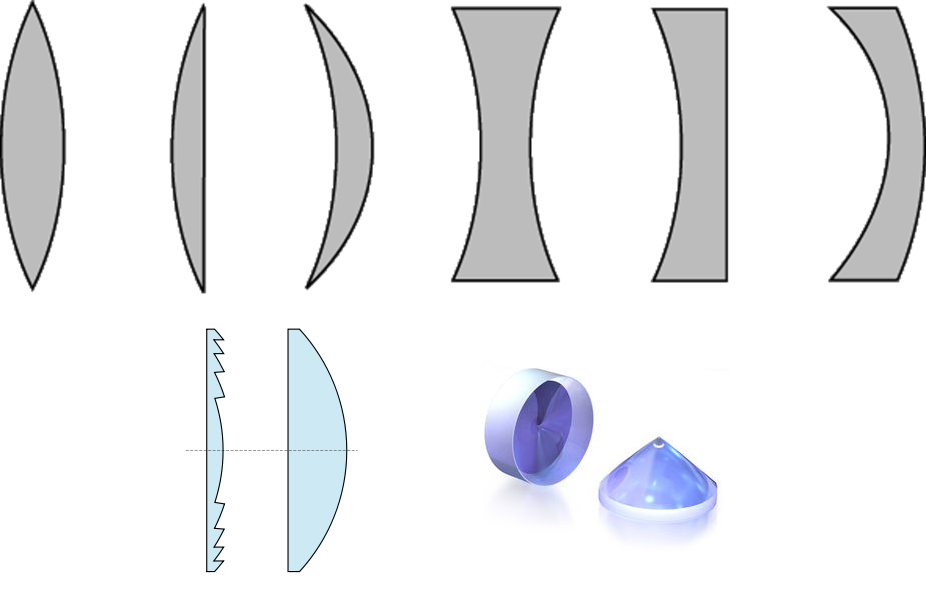
\includegraphics[width=1\textwidth]{5lenses.png}
	\label{pic:5lenses}
\end{figure}

Форма боковой поверхности линзы чаще всего выполняется круглой (цилиндрической), что является наиболее технологичным при изготовлении и закреплении в оправе (иногда форма боковой поверхности выполняется прямоугольной или сегментарной).

\textbf{Конструктивные параметры} линз подразделяют на \textit{расчетные} и \textit{конструкторские}.

К \textit{расчетным параметрам} (рис.~\ref{pic:5draw},~\ref{pic:5faska}) относят оптические характеристики и показатели качества материала линзы, ее световые диаметры на рабочих поверхностях (диаметр поверхности линзы, пропускающей световой поток), толщину линзы по оптической оси, радиусы кривизны (или параметры формы) преломляющих поверхностей, фокусное расстояние и вершинные фокальные отрезки, допустимые значения погрешностей изготовления оптических поверхностей (погрешности формы, децентрировку\footnote{Децентрировка -- несовпадение оптической оси линзы с геометрической осью}, отклонение толщины по оси), вид оптических покрытий. Эти данные определяются при габаритном, аберрационном, светотехническом расчетах оптической системы.

К \textit{конструкторским параметрам} (рис.~\ref{pic:5draw}--\ref{pic:5lensdraw}), относят полный диаметр линзы (или ее размеры, при некруглой форме), параметры фасок, толщину по краю, габаритный размер вдоль оси, чистоту рабочих и шероховатость нерабочих поверхностей, вид покрытия нерабочих (матовых) поверхностей, допуски на погрешности не справочных параметров. Эти параметры определяют в процессе конструирования при окончательном оформлении ее конструкции.

\begin{figure}[h!]
	\caption{Чертеж линзы без защитных фасок}
	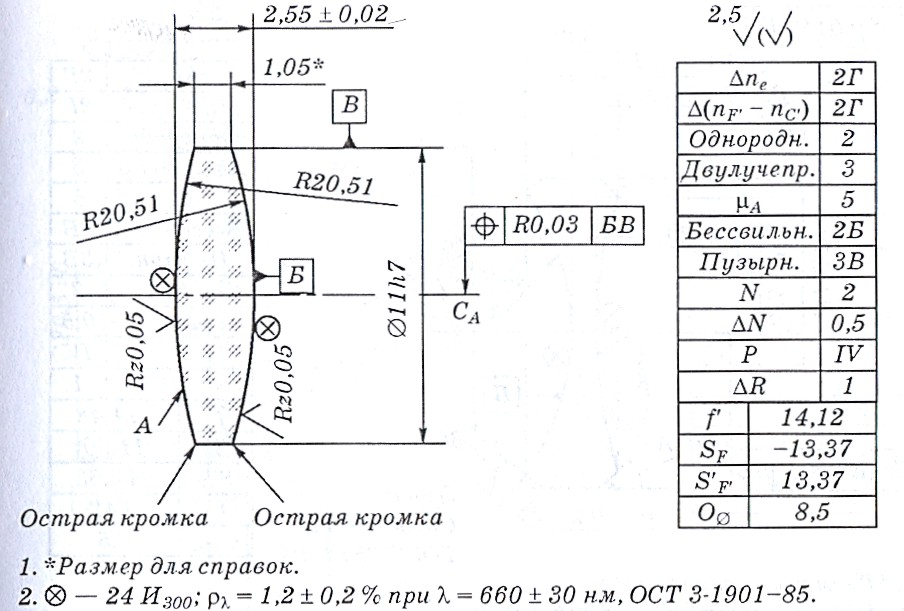
\includegraphics[width=1\textwidth]{5draw.png}
	\label{pic:5draw}
\end{figure}

\begin{figure}[h!]
	\caption{Линза с конструктивной фаской}
	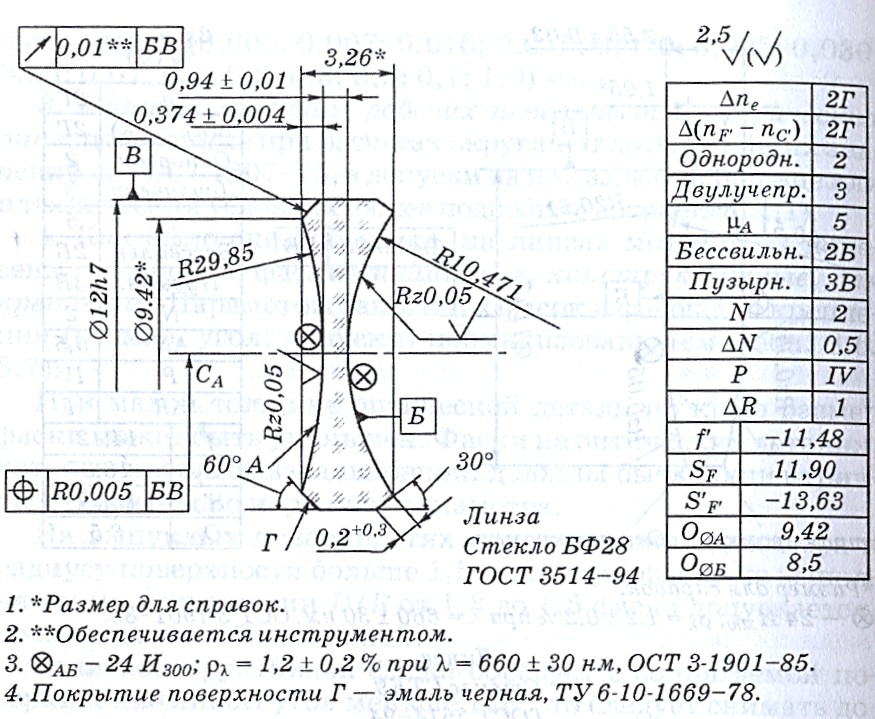
\includegraphics[width=1\textwidth]{5faska.png}
	\label{pic:5faska}
\end{figure}

Рассмотрим некоторые аспекты определения конструктивных параметров.
\begin{enumerate}
	
\item Для закрепления линзы в оправе ее полный диаметр выполняют несколько больше светового. Минимальное значение полного диаметра линзы зависит от светового диаметра и способа закрепления. Окончательный размер полного диаметра округляется до ближайшего (большего) нормального диаметра по действующим стандартам. Поля допусков на полный диаметр линзы должны образовывать в соединении с оправой линзы посадку с зазором, поэтому в зависимости от необходимого значения гарантированного зазора и точности центрирования обычно проставляют следующие допуски на диаметры линз:

$ g6, f7 $ -- высокая точность (технический уровень точности);
$ h8, f9, e9 $ -- средняя точность (производственный уровень точности);
$ d9, c11, d11 $ -- пониженная точность (экономический уровень точности).

Заметим, что в соединении линзы с оправой должен быть обеспечен необходимый <<температурный>> зазор, а также то, что точность центрировки линзы в оправе зависит не только от допуска на ее диаметр, но и от выполнения условия самоцентрирования и использования результативной обработки оправы после закрепления линзы.

\item Исходя из требований технологии при конструировании положительных линз необходимо обеспечивать минимальную толщину по их краю в соответствии с рекомендациями, приведенными в соответствующих справочных материалах, а толщина по оси отрицательных линз в зависимости от ее диаметра и необходимой точности формы рабочих поверхностей должна соответствовать рекомендациям действующих стандартов (в пределах от $ 0,05D $ до $ 0,09D  $ в зависимости от диаметра линзы).

Рассчитанные предельные допуски на толщину линз вдоль оси (исходя из их влияния на качество изображения) округляют до ближайшего меньшего значения из ряда значений, приведенного в действующих стандартах [$ \pm(0,005; 0,007; 0,010; 0,015; 0,020; 0,025; 0,030-0,05; 0,07; 0,1; 0,2; 0,3; 0,5; 0,7; 1,0) $ мм].

\item Радиусы кривизны рабочих поверхностей сферических линз, полученные при расчетах, округляют до ближайших значений по действующим стандартам, а допуски на них задают в таблице или в технических условиях.

\item На линзах могут быть нанесены следующие фаски (рис.~\ref{pic:5faska}): защитные, конструктивные, для крепления. Параметры защитных фасок и фасок для крепления (размер, угол, допуски) нормализованы (приведены в соответствующих таблицах).

При малой толщине оптической детали по краю размер фаски может быть уменьшен. Фаски на оптических деталях, которые крепятся завальцовкой, должны быть концентричны относительно наружного диаметра.

На выпуклых поверхностях при отношении диаметра к радиусу поверхности больше 1,5 защитную фаску не выполняют; при отношении $ D/R $ от 1,3 до 1,5 фаска допускается, но не является обязательной.

На некоторых линзах, собранных в линзовую систему групповым способом <<насыпным без промежуточных колец>>, защитные фаски на кромках не снимают. Обусловлено это тем, что при применении данного способа крепления линзы в системе устанавливаются друг по другу рабочими поверхностями и кромками (фасками), поэтому значительные погрешности защитных фасок вызывают погрешности воздушных промежутков между компонентами и нарушают центрировку линз в системе (рис.~\ref{pic:5draw}).

Для точной центрировки линзы и обеспечения номинального расстояния между компонентами на соответствующей кромке линзы выполняется конструктивная фаска, которая может быть нанесена не вручную, а при помощи инструмента с последующим контролем ее размера (расположения) и биения (рис.~\ref{pic:5faska}).

\item В качестве материала для линз используется в основном оптическое стекло различных марок. Однако в последнее десятилетие широкое применение получили линзы из оптических полимеров (полиметилметакрилат, полистирол, поликарбонат, сополимер, zeonex), в частности в массовом производстве линз фотографической техники широкого потребления, линз осветительных систем (например, линз Френеля), очковых линз, линз окуляров, лупы, что существенно облегчает их массу и уменьшает стоимость.

Линзы, работающие в инфракрасной и ультрафиолетовой областях спектра, изготавливаются из специальных марок стекол (К515, ИКС), кварцевого стекла (КУ-1), оптической керамики, оптических кристаллов (флюорита, сильвина, фтористого лития, германия).

\item Оптические характеристики линзы: $ f, f' $ -- фокусные расстояния (переднее и заднее); $ S_F, S'_{F'} $  -- передний и задний фокальные отрезки; и расчетные световые диаметры на рабочих поверхностях линз указывают в третьей части таблицы, причем один из фокальных отрезков при необходимости может указываться с допуском.

\item Допуск на децентрировку рабочей поверхности линзы выражают в долях миллиметра и проставляют в поле чертежа, в специальной рамке, содержащем три поля, в первом указывают значок вида допуска децентрировки (позиционный, перпендикулярности или биения плоской поверхности, формы заданной поверхности), во втором -- численное значение допуска, в третьем указывают базы, относительно которых следует контролировать децентрировку (рис.~\ref{pic:5draw}, \ref{pic:5faska}).

При контроле децентрировки круглую линзу (или линзовый блок) устанавливают одной из базовых поверхностей на кольцевую опору, поджимают другой базовой поверхностью к ножевидному упору и приводят во вращение. Измеренное при этом биение центра кривизны рабочей поверхности (или биение плоской поверхности) относительно базовой оси (создаваемой базовыми поверхностями) является мерой децентрировки. Контроль децентрировки некруглых сферических линз, цилиндрических и асферических линз производится с помощью специальных методов и приборов.

Высокий уровень точности центрировки линз соответствует значениям их децентрировки в диапазоне 0,002-0,005 мм, среднему уровню соответствует диапазон 0,005-0,01 мм и пониженному уровню -- 0,01-0,02 мм.

\item На рабочие  поверхности  линзы  могут  быть нанесены различные виды оптических покрытий (просветляющих, зеркальных, светоделительных и поглощающих), а для уменьшения бликов и защиты детали от влияния внешней среды выполняют покрытия их боковых поверхностей и фасок.
\end{enumerate}

\begin{figure}[h!]
	\caption{Чертеж линзы без защитных фасок}
	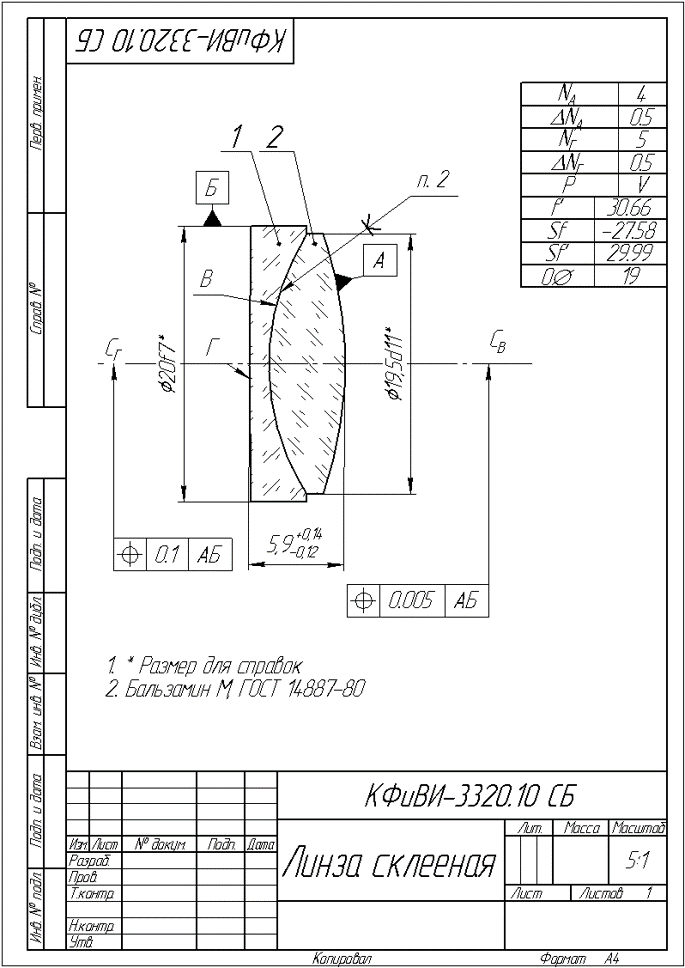
\includegraphics[width=0.7\textwidth]{5lensdraw.png}
	\label{pic:5lensdraw}
\end{figure}

Одиночные сферические линзы вследствие больших аберраций редко применяются как самостоятельные элементы оптических приборов. Чаще используются комбинации из нескольких линз, склеенные линзы (склейки, линзовые блоки), выполняющие те же функции, что и одиночные линзы, но со значительно меньшими аберрациями.

Большое распространение в ОЭП получили склеенные блоки из двух линз (реже трех линз и более) -- положительной и отрицательной, изготовленные из стекол различных марок типа крон и флинт (рис.~\ref{pic:5skleyka}). Они применяются, например, в качестве объективов и оборачивающих линз телескопических приборов. У двухлинзовых склеек могут быть хорошо исправлены сферическая аберрация, хроматизм и кома, другие же аберрации устранить достаточно полно невозможно.

\begin{figure}[h!]
	\caption{Склейки линз}
	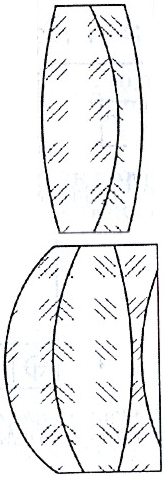
\includegraphics[width=0.5\textwidth]{5skleyka.png}
	\label{pic:5skleyka}
\end{figure}

Для склеивания линз (и других оптических деталей) применяют специальные оптические клеи: пихтовый бальзам, бальзамин, бальзамин-М, акриловый, УФ-215М, эпоксидный и другие оптические клеи, которые обладают рядом необходимых свойств и характеристик (высокая прозрачность в спектральном диапазоне, близость показателя преломления к показателям преломлений склеиваемых материалов, оптическая однородность, отсутствие возникновения существенных напряжений при полимеризации, стабильность свойств во времени, тепло- и морозостойкость).

Основные марки оптических клеев и их свойства приведены в действующих стандартах, рекомендации по использованию тех или иных марок клеев при склеивании линз и других оптических деталей в зависимости от условий их работы приведены в соответствующих справочниках.

Чертеж линзового блока оформляется в соответствии с требованиями, приведенными ранее. На чертеже блока, являющегося сборочной единицей, указываются только те параметры, которые должны быть выполнены и проконтролированы в процессе сборки (склейки): центрировка и толщина склеенного блока, отсутствие деформаций наружных рабочих поверхностей, их чистота. Поэтому верхняя часть таблицы -- требования к материалу -- на чертеже склеенного блока линз отсутствует, таблица состоит только из двух частей: требований к сборке и оптических характеристик.

В склейке одна из линз является базовой, а другая -- присоединяемой (приклеиваемой). При конструировании деталей, входящих в склейку, как правило, на полный диаметр базовой линзы назначается допуск $ e9 $, для приклеиваемой -- $ d10 $ или $ d11 $. Допускается выполнять приклеиваемую линзу с уменьшенным диаметром по номиналу по сравнению с базовой линзой на 0,2 -- 0,4~мм на диаметр.

При определении базовой и приклеиваемой линз следует учитывать следующее:
\begin{itemize}
\item в качестве базовой следует выбирать линзу с большей толщиной по краю для удобства базирования при склеивании и контроле готового узла;
\item в качестве базовой следует выбрать ту деталь, у которой в склейку идет вогнутая поверхность, поскольку клей при склеивании не должен вытекать из соединительного шва, а напротив, должен заполнять все образующиеся пустоты при сопряжении двух линз;
\item наружный радиус базовой линзы желательно иметь большего значения, чем наружный радиус приклеиваемой линзы для более точного и удобного изготовления склейки;
\item желательно, чтобы показатель преломления материала базовой линзы не значительно отличался от показателя преломления клея по сравнению с разницей показателей преломления клея и материала приклеиваемой линзы;
\item необходимо, чтобы радиус базовой поверхности был больше радиуса приклеиваемой поверхности (это касается как базовой, так и приклеиваемой линз);
\item желательно, чтобы базовая поверхность базовой линзы оставалась базовой поверхностью и для всей склейки;
\item желательно, чтобы у приклеиваемой линзы базовой являлась та поверхность, которая уходит в склейку.
\end{itemize}

Допуск на децентрировку базовой линзы ставится более жесткий, чем допуск на приклеиваемую линзу. Особенно это касается случая, когда показатель преломления материала приклеиваемой линзы фактически совпадает с показателем преломления клея.

Допуск на суммарную толщину склейки линз рассчитывается следующим образом: \\ $ \Delta d_\text{скл} = \Delta d_\text{баз} + \Delta d_\text{прик} + 0,01$ , например:
\[ d_\text{баз} = 1 \pm 0,01; \]  
\[ d_\text{пр} = 4 \pm 0,02; \] 
\[ d_\text{скл} = 1_{-0,01}^{+0,01}  + 4_{-0,01}^{+0,01} + 0,01 = 5. \]

На наружные рабочие поверхности склейки линз могут быть нанесены оптические покрытия, а боковые поверхности и фаски (матовые поверхности) покрывают защитными эмалями.

\section{Общие требования к оптическим узлам и устройствам}
Сборочные единицы, выполняющие в приборе определенные функции только совместно с другими составными частями, но объединенные в процессе проектирования и изготовления (сборки) в единую систему, называются конструктивными узлами. Они обычно состоят из относительно небольшого количества сопряженных друг с другом деталей, среди которых выделяют рабочую, базовую (оправу, корпус) и вспомогательные (крепежные, ориентирующие, технологические). 

Типичными представителями конструктивных узлов оптических приборов являются узлы крепления оптических деталей и узлы фотоприемников. Прежде чем рассмотреть типовые конструкции таких узлов, перечислим некоторые общие требования к ним и состоящим из них функциональным устройствам.

\begin{enumerate}
	
\item Конструкция узла должна обеспечить точное расположение рабочей детали (ее рабочих элементов) относительно базовой детали (базового элемента оправы).

\item Крепление должно быть надежным; не допускается изменение положения рабочей детали относительно оправы после закрепления в процессе эксплуатации.

\item В конструкции не должно возникать опасных (объемных) деформаций рабочей и базовой деталей и внутренних напряжений в них при закреплении и в процессе эксплуатации.

При силовом замыкании крепежные элементы не должны вызывать деформации изгиба или кручения. Допускается деформация сжатия (контактная). Для уменьшения деформаций из-за погрешностей размеров, формы и положения элементов деталей между крепежной деталью и оптической следует устанавливать упругие или эластичные прокладки (металлические пружинные кольца, прокладки из пробки, картона, поранита).

Обязательно должно быть обеспечено отсутствие температурных деформаций (или смещений рабочей детали относительно базовой) при перепадах температуры.
\item Конструкция узла при необходимости должна обеспечивать возможность юстировки рабочей детали. Потребность в юстировке может быть нужна в двух случаях: для точного расположения рабочей детали относительно оправы (например, центрирование линзы при ее сборке относительно базовой оси оправы); для обеспечения требуемого расположения рабочей детали относительно рабочих деталей или баз других узлов (например, фокусировка линзы на фотоприемник). Поэтому для первого случая конструкция узла должна обеспечивать юстировочные подвижки рабочей детали относительно оправы в процессе ее закрепления, для второго~-- подвижки рабочей детали в оправе или вместе с ней (т.е.~всего узла) относительно других узлов в процессе либо после сборки функционального устройства или всего прибора.

\item Конструкция узла должна быть технологичной в отношении изготовления деталей и особенно в отношении их сборки (свободный доступ инструмента, возможность автоматизации сборки, удобство контроля, доступность и простота обслуживания и замены малонадежных элементов).

\item Габаритные размеры узла желательно минимизировать, чтобы обеспечить отсутствие срезания пучка лучей, появление бликов и рассеянного света в системе.

\item Конструкции функциональных устройств должны быть унифицированы по принципам построения, целевым характеристикам, присоединительным размерам, номиналам электропитания.

\item Фактически ни одно функциональное устройство не обходится без юстировки его показателей качества, поэтому надо знать необходимые юстировочные операции типовых функциональных устройств, методику их выполнения (с перечнем необходимого контрольного оборудования), уметь рассчитывать требования к юстировке и заложить в конструкции устройств возможность ее осуществления.

\end{enumerate}

Выполнение перечисленных требований основывается на использовании принципов и правил конструирования соединений, узлов и функциональных устройств.

%\section{Конструкции узлов крепления круглых оптических\\ деталей и линзовых систем}

К основным способам крепления линз и других круглых оптических деталей относятся: крепление завальцовкой, крепление приклеиванием, крепление резьбовым кольцом. При необходимости, когда приходится учитывать особые условия и требования, связанные с габаритными размерами, назначением, условиями эксплуатации оптических деталей, могут использоваться вспомогательные способы крепления: проволочным кольцом, прижимными планками, накладным кольцом, специальными элементами или специальной конструкцией оправы. Указанные названия способов крепления определены видом замыкания рабочей (оптической) детали с базовой (оправой) в соединении или видом крепежной детали.

\begin{flushleft}
	\textbf{Крепление завальцовкой}
\end{flushleft}

При этом способе крепления линза поджимается к опорному уступу тонким буртиком, выполненным на оправе. Операция завальцовки производится на токарном или сверлильном станках при помощи роликов, специальных инструментов или ультразвуком. В результате тонкий буртик оправы (рис.~\ref{pic:5zavalcovka}) деформируется и загибается по всей окружности на специально выполненную фаску линзы.

\begin{figure}[h!]
%	\caption{Крепление линзы завальцовкой:\\ а -- размеры, буртика; б -- общий вид}
	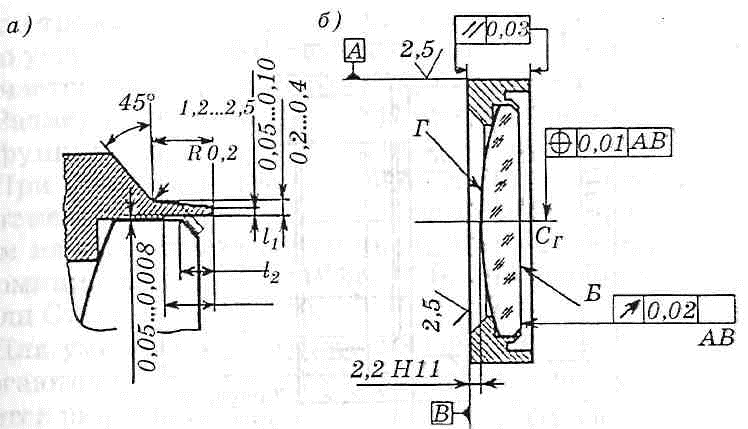
\includegraphics[width=1\textwidth]{5zavalcovka.png}
	\label{pic:5zavalcovka}
\end{figure}

Чтобы не образовалось сколов кромки линзы при загибании буртика, на внутренней поверхности оправы выполняют выборку $ l_2 $. Размеры элементов загибаемого буртика берутся из справочника конструктора оптико-механических приборов. 

Преимуществами этого метода крепления являются простота и компактность конструкции соединения. Закрепляющий тонкий буртик, обладая упругими свойствами, обеспечивает силовое замыкание линзы без напряжений, а также компенсирует температурные деформации. Возможна автоматизация сборки соединения. Кроме того, в процессе завальцовки линзы можно выполнять ее частичную центрировку.

Недостатки: конструкция неразборная; существует ограничение на массу закрепляемой линзы (склеенного блока). Ограничение объясняется тем, что тонкий (до 0,1 мм) загибаемый буртик не обеспечивает надежного крепления массивных линз. Выполнение буртика большей толщины исключает его упругие свойства и может привести к выколкам кромки линзы в процессе завальцовки и ухудшить эксплуатационные свойства соединения. Поэтому крепление завальцовкой рекомендуется применять для линз от 6 до 80 мм, а склеенных блоков -- до 50 мм.

Технология завальцовки предполагает наличие специальных оборудования, приспособлений и определенной квалификации сборщика. Точность центрирования линзы в оправе может быть несколько ниже, чем при других способах крепления из-за того, что закрепляющий буртик ложится на матовую поверхность нецентрированной фаски линзы.

При креплении завальцовкой для оправ обычно используют легко деформируемые, но упругие материалы. Наилучшим из них является латунь ЛС59-1. Также применяются алюминиевые сплавы Д1, Д6, Д16, В95 и низкоуглеродистые стали Сталь 20, Сталь 30.

Для уменьшения отражения света от стенок оправы подвергаются чернению, а на внутренних поверхностях выполняется рифление.

Завальцовка иногда используется при креплении несклеенных блоков (состоящих из двух-трех) линз и весьма часто -- при креплении сеток, светофильтров, защитных стекол и других деталей, имеющих круглую форму.

\begin{flushleft}
	\textbf{Крепление приклеиванием}
\end{flushleft}

В настоящее время способ крепления линз и других круглых оптических деталей приклеиванием к оправам является все более и более используемым. Причиной этому служит появление новых клеящих веществ с оптимальными свойствами для соединения оптических деталей с оправами (обеспечение надежности соединения, эластичность, отсутствие деформаций в слоях клея, хорошая адгезия к различным материалам, способность сохранять свойства при внешних воздействиях, стабильность во времени).

В результате данные узлы крепления имеют ряд положительных качеств:
\begin{itemize}
\item конструктивная простота узла крепления, а также снижение его массы и габаритных размеров;
\item возможность закрепления линз, крепление которых традиционными способами затруднено, например линз малого диаметра (до 6~мм), с крутыми радиусами кривизны и тонкими краями (рис.~\ref{pic:5glue}), при некруглой форме базовых поверхностей;
\item отсутствие деформаций и напряжений в оптической детали при внешних воздействиях на узел крепления (например, при изменении температуры) благодаря упругим свойствам клеящих веществ;
\item возможность корректировки положения оптической детали до момента затвердевания клеящего вещества;
\item обеспечение герметизации соединения;
\item относительная простота автоматизации процесса сборки.
\end{itemize}

\begin{figure}[h!]
	\caption{Крепление линз объектива приклеиванием}
	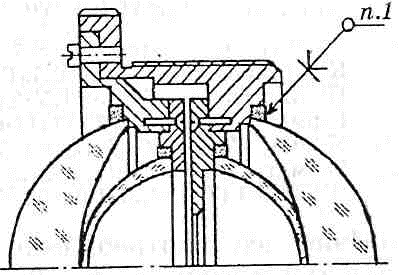
\includegraphics[width=0.6\textwidth]{5glue.png}
	\label{pic:5glue}
\end{figure}

Заметим, что этот способ наиболее часто применяется также для крепления линз приклеиванием в случаях, когда они имеют некруглую форму боковых поверхностей.

Качество соединения линзы с оправой зависит от согласованности материалов, входящих в узел крепления компонентов. Для этого необходимо знать физико-механические свойства клеящего вещества, линзы и оправы.

Материал, из которого изготовлены линзы для последующего крепления приклеиванием, может быть любым. Чистота обработки поверхности стекла в месте крепления не оказывает существенного влияния на скрепляющее свойство. Поэтому приклеиваемая поверхность линзы может быть шлифованной.

Оправы, к которым приклеиваются линзы, изготавливают из алюминиевых сплавов, латуни, стали, титана и его сплавов: ВТ1-0, ОТ4, ВТ-5, ВТ-16. Из перечисленных материалов титан благодаря тепловым свойствам, близким к стеклу, является наиболее оптимальным для изготовления оправ линз. Особенность оправ -- их антикоррозийное покрытие (химическое оксидирование для сталей и анодное оксидирование для цветных металлов).

На чертежах в соответствии с ГОСТ~2.313-82 клеевые швы изображают жирной линией (на разрезах это может быть некоторая область). К этой линии подводят выноску, на которой ставят знак К (рис.~\ref{pic:5glue}).

\begin{figure}[h!]
%	\caption{Крепление линз приклеиванием: \\а -- с базированием на рабочие элементы оправы; б -- с базированием на клеевой шов; в -- с комбинированным базированием}
	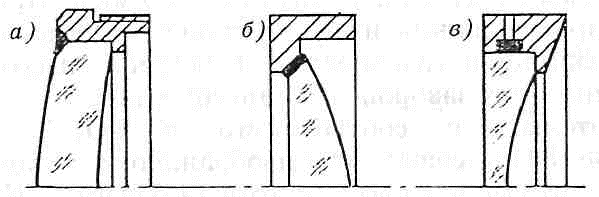
\includegraphics[width=1\textwidth]{5glue1.png}
	\label{pic:5glue1}
\end{figure}

На рис.~\ref{pic:5glue1} показаны три типовые конструкции крепления одиночных линз приклеиванием. Мениск базируется в отверстие на уступ оправы (рис.~\ref{pic:5glue1}~а). Закрепляющий клеевой шов образуется за счет заполнения клеем сопряженных фасок на линзе и оправе. Плосковыпуклая линза устанавливается фаской на клеевой шов (рис.~\ref{pic:5glue1}~б), который наносится на рабочую поверхность оправы. Плосковогнутая линза базируется на уступ оправы в осевом направлении (рис.~\ref{pic:5glue1}~в). Для образования клеевого шва в посадке линзы и оправы выполняется увеличенный до 0,5 мм зазор, так как очень тонкие слои клея теряют упругие свойства. При невозможности увеличить толщину клеевого слоя между линзой и оправой (например, для повышения точности базирования) в последней выполняется специальная канавка, которая заполняется клеем (рис.~\ref{pic:5glue1}~в).

Способ крепления оптических деталей приклеиванием имеет некоторые недостатки. Увеличение объема или усадка клеящего вещества после отвердевания могут вызвать напряжения в линзе. Поскольку зазор между линзой и оправой заполнен клеящим веществом, то при перепадах температур, из-за различных расширений этих деталей, возможно расклеивание или возникновение напряжений и деформаций. 

Большая длительность сушки клеящих веществ (от нескольких часов до суток) требует особой технологии, снижает производительность сборки. Некоторые компоненты клеящих веществ при определенных условиях (в вакууме) начинают испаряться, что может привести к загрязнению линз. Крепление, как правило, неразборное, поэтому не подлежит восстановлению. Базирование линзы в оправе на клеевой шов (рис.~\ref{pic:5glue1}~б) не обеспечивает высокую точность ее положения. Крепление линз и склеек с большой массой недостаточно надежно и требует его дублирования прижимными деталями.

Влияние ряда недостатков может быть уменьшено. Например, для повышения точности расположения линз в конструкции узла необходимо предусмотреть базирование линзы непосредственно на рабочие поверхности оправы (рис.~\ref{pic:5glue1}~а). 

В целом, несмотря на указанные недостатки, способ крепления линз приклеиванием имеет много положительных свойств, выгодно отличающих его от других, главным образом благодаря конструктивной простоте, экономичности, надежности и возможности автоматизации сборки.

\begin{flushleft}
	\textbf{Крепление резьбовым кольцом}
\end{flushleft}

Применяется как разъемное крепление отдельных линз, склеенных и составных линзовых блоков и других круглых оптических деталей. Оптическая деталь прижимается к опорному уступу оправы кольцом, имеющим наружную (или внутреннюю) резьбу, по которой оно завинчивается в оправу (рис.~\ref{pic:5ring} а). Кольцо завинчивается в оправу специальным ключом, вставляемым в специально выполненные шлицы или отверстия, а для кольца с внутренней резьбой выполняется накатка (рис.~\ref{pic:5ring}~б).

\begin{figure}[h!]
%	\caption{ Крепление линзы резьбовым кольцом:\\ а -- кольцо с наружной резьбой; б -- кольцо с внутренней резьбой}
	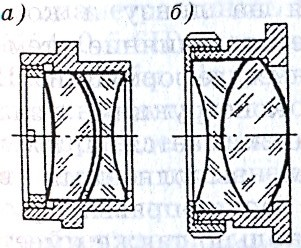
\includegraphics[width=0.5\textwidth]{5ring.png}
	\label{pic:5ring}
\end{figure}

Резьбовым кольцом рекомендуется крепить линзы с диаметром свыше 10 мм вследствие технологических трудностей выполнения внутренней резьбы в оправах меньшего диаметра, а также из-за относительно больших (по сравнению с размером линзы) габаритных размеров кольца.

Преимуществами данного способа являются обеспечение надежного разъемного крепления, простота сборки и демонтажа, отсутствие ограничений крепления линз относительно большого диаметра (до 300 мм). 

К недостаткам относятся следующие:
\begin{itemize}
\item конструкция менее технологична, чем при креплении завальцовкой или приклеиванием (так как требуется наличие дополнительной детали, крепежной резьбы в оправе, необходимо предохранять резьбовое кольцо от самоотвинчивания);
\item узел имеет увеличенные, особенно в осевом направлении, габаритные размеры; затруднена автоматизация сборки соединения;
\item невозможна юстировка линзы в оправе в процессе сборки;
\item не всегда можно обеспечить равномерный по всей окружности прижим линзы к опорному уступу оправы, что связано с перекосами кольца в резьбовом соединении, погрешностями формы и положения (отклонение от перпендикулярности) торца кольца и опорного уступа, разнотолщинностью (клиновидностью) линзы по краю;
\item при работе соединения в условиях перепада температур, из-за его жесткости могут возникнуть либо деформации линзы, либо смещения из-за уменьшения усилия прижатия или даже возникающего зазора между линзой и резьбовым кольцом.
\end{itemize}

Для устранения последних недостатков между резьбовым кольцом и линзой устанавливают пружинное кольцо (рис.~\ref{pic:5ring1}). Вследствие упругости кольца в осевом направлении достигается равномерное по всей окружности распределение давления на линзу и компенсируется влияние температурных деформаций. 

В данной конструкции узла линза поджимается к трем выступам, выполненным в опорном торце оправы. Пружинное кольцо также имеет три выступа, которые ориентированы напротив выступов оправы с помощью винта I, позволяющего   пружинному кольцу смещаться вдоль оси, но ограничивающего его разворот. В результате достигается геометрическая определенность соединения, что обеспечивает минимальные деформации при прижиме.

\begin{figure}[h!]
	\caption{ Крепление линзы с установкой пружинного кольца }
	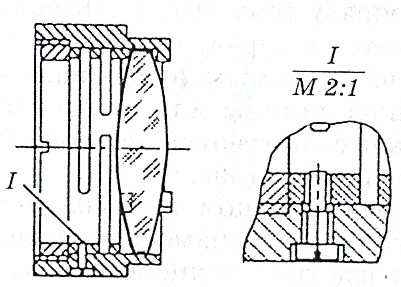
\includegraphics[width=0.65\textwidth]{5ring1.png}
	\label{pic:5ring1}
\end{figure}

\begin{flushleft}
	\textbf{Крепление проволочным кольцом}
\end{flushleft}

Этот способ применяется для закрепления линз диаметром 20-80~мм при невысоких требованиях к точности их центрирования и герметичности соединения. Он используется в основном для закрепления линз и зеркал в осветительных системах и не силовых оптических деталей (светофильтров, защитных стекол, матовых и молочных рассеивателей).

На рис.~\ref{pic:5ring2} изображены два варианта крепления линзы проволочным кольцом. В первой конструкции (рис.~\ref{pic:5ring2}~а) линза помещена между опорным уступом и выступающей частью проволочного кольца, установленного в прямоугольную кольцевую канавку оправы. Ширина канавки равна диаметру (толщине) проволоки, а глубина -- половине диаметра. Кольцо имеет вырез и изготавливается из стальной углеродистой пружинной проволоки (иногда латунной или бронзовой) диаметром 0,4--1,0мм (рис.~\ref{pic:5ring2}~в).

\begin{figure}[h!]
%	\caption{ Крепление проволочным кольцом:\\ а -- оправа с прямоугольной канавкой; б -- оправа с конической канавкой;\\ в -- проволочное кольцо }
	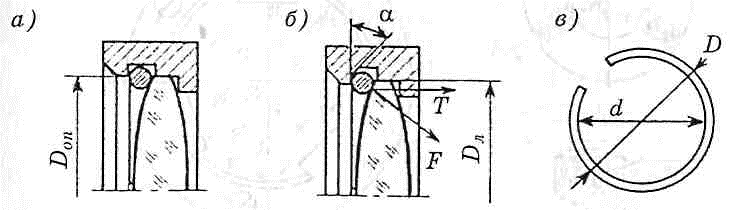
\includegraphics[width=1\textwidth]{5ring2.png}
	\label{pic:5ring2}
\end{figure}

Условие установки проволочного кольца в оправу: $ D_{min} < D_\text{оп} $, где $ D_{min} $ -- диаметр сжатого кольца; $ D_\text{оп} $ -- диаметр отверстия оправы; а условие крепления линзы в оправе: $ d_{max} < D_\text{л} $, где $ d_{max} $ -- внутренний диаметр кольца, установленного в оправу; $ D_\text{л} $ -- диаметр линзы.

Крепление проволочным кольцом конструктивно простое и технологичное. Кольцо может быть быстро установлено или снято.

Недостатком такого способа крепления является возможность смещения и перекашивания линзы в оправе, которые возникают из-за осевого зазора (обусловленного погрешностями размеров канавки, толщины линзы по краю, диаметра проволоки).

Во второй конструкции в оправе выполнена конусная канавка под проволочное кольцо (рис.~\ref{pic:5ring2}~б). В месте контакта кольца с наклонной плоскостью канавки возникает сила реакции, осевая составляющая которой прижимает линзу к опорному уступу. Для надежности соединения угол   конусной канавки должен быть меньше угла трения.

\begin{flushleft}
	\textbf{Крепление пружинящими планками}
\end{flushleft}

Крепление при помощи пружинящих планок применяется для линз, работающих в условиях перепадов температур, динамических воздействий и в случаях, когда они имеют не круглую форму боковых поверхностей. Упруго деформируясь, планки компенсируют действие факторов, ухудшающих качество соединения. Пример крепления пружинящими планками показан на рис.~\ref{pic:5planka}.

\begin{figure}[h!]
%	\caption{ Крепление пружинящими планками:\\ а -- тремя планками; б -- кольцевой планкой }
	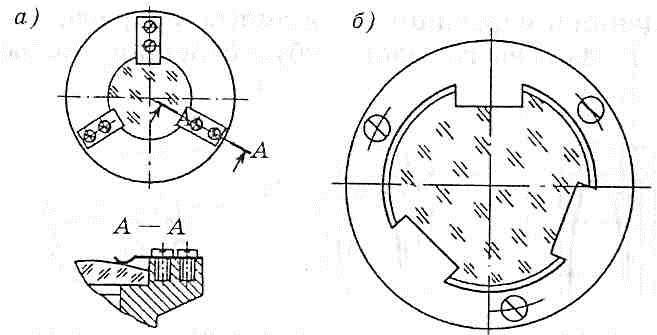
\includegraphics[width=1\textwidth]{5planka.png}
	\label{pic:5planka}
\end{figure}

Планки изготавливают из лент холоднокатаной инструментальной или пружинной стали (65Г, У8А), нейзильбера (НМцб5-20) и устанавливают через 120$^\circ$ по окружности оправы, как показано на рис.~\ref{pic:5planka}~а. Каждая планка привинчивается к оправе двумя винтами.

Для крепления линз малого диаметра три планки заменяют одним кольцом с тремя пружинящими выступами (рис.~\ref{pic:5planka}~б). Возможны и другие конструктивные реализации пружинящих планок и их соединений с оправой.

Конструкция узла характеризуется достаточной точностью и надежностью соединения линзы с оправой.

Преимуществами, которыми обладает данный способ крепления, являются следующие: возможность регулировать усилие прижима; создание упругого соединения, позволяющее компенсировать погрешность осевых размеров сопрягаемых деталей и их изменение от внешних воздействий; возможность разборки конструкции; отсутствие необходимости в специальном оборудовании и квалифицированном персонале для сборки узла. К недостаткам следует отнести: нетехнологичность конструкции, содержащей большое количество крепежных элементов; сложность автоматизации сборки; невозможность юстировки в процессе сборки.

\begin{flushleft}
	\textbf{Крепление накладным кольцом}
\end{flushleft}

Данный способ применяют для крепления крупногабаритных линз, а также других круглых оптических деталей (защитных стекол, зеркал) с диаметром, превышающим 200-300~мм. Крепление накладным кольцом относится к индивидуальным способам крепления. Его реализация зависит от конкретных геометрических параметров оправы и линзы, их допустимых отклонений, а также от температурного режима работы соединения.

Схема крепления показана на рис.~\ref{pic:5nakladnoe}. Линзу устанавливают в оправу на фаску опорного буртика, выполненную под углом 135$^\circ$ или по касательной к рабочей поверхности линзы, к которому она прижимается накладным кольцом. Рабочая поверхность прижимного кольца тоже выполняется по касательной к поверхности линзы и крепится к оправе болтами Для компенсации погрешностей изготовления соответствующих размеров оправы, линзы и накладного кольца и их изменений при отклонениях температуры между контактирующими поверхностями линзы и кольца устанавливается упругая прокладка.

\begin{figure}[h!]
	\caption{ Крепление линзы накладным кольцом }
	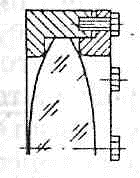
\includegraphics[width=0.3\textwidth]{5nakladnoe.png}
	\label{pic:5nakladnoe}
\end{figure}
 
Для центрирования линзы в оправе могут применяться вкладыши (например, полоски фольги толщиной 0,005 мм), которые устанавливают в зазор между посадочным отверстием оправы и линзой. Иногда линзу центрируют в оправе сдвигом (наклоном) винтами с последующей фиксацией герметиком.
Для компенсации возможных пережатий или смещений линзы при перепадах температуры в ряде случаев между диаметрами линз и отверстиями оправы устанавливают термокомпенсаторы.

Данный способ крепления обладает рядом недостатков: трудоемкость сборки узла из-за подгонки прижимного кольца; увеличенные габаритные размеры конструкции, так как накладное кольцо выступает за пределы оправы; невозможность автоматизации сборки.

К преимуществам способа следует отнести: надежность крепления; возможность частичной юстировки положения линзы относительно оправы; возможность применения термокомпенсаторов.

\begin{flushleft}
	\textbf{Специальные (нетрадиционные) способы крепления}
\end{flushleft}

К этим способам крепления линз относятся, например: крепление линзы в оправе стопорными винтами (или привинчивание линзы винтами к оправе через просверленные в ней отверстия); заливка линзы в оправе зубным или глетоглицериновым цементом; заформовка линзы в оправу из термопластичных пластмасс; обжатие линзы <<хомутовыми>> или разъемными оправами. На рис.~\ref{pic:5obj} изображена конструкция проекционного объектива, линзы которого закреплены в разъемной пластмассовой оправе.

\begin{figure}[h!]
	\caption{ Проекционный объектив }
	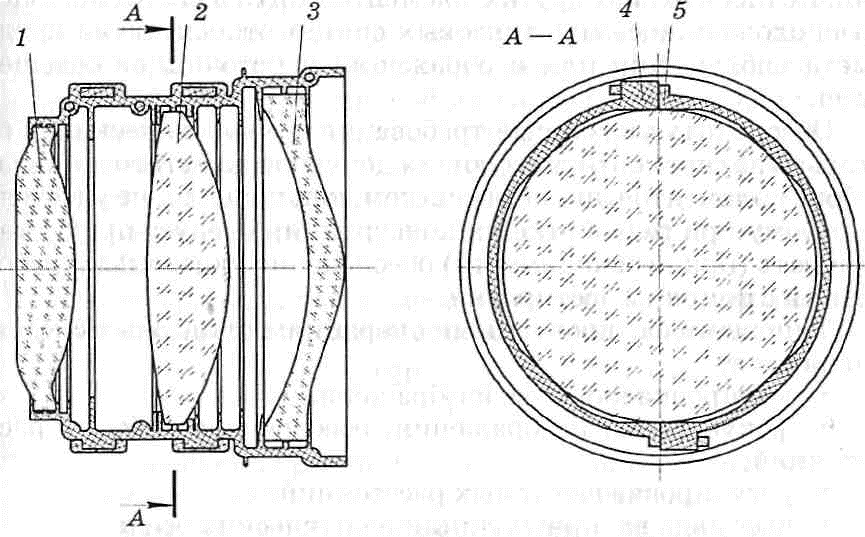
\includegraphics[width=1\textwidth]{5obj.png}
	\label{pic:5obj}
\end{figure}

\section{Конструкции линзовых систем}

К линзовым системам оптических приборов относятся объективы, окуляры, оборачивающие системы, системы смены увеличения, конденсоры и коллекторы. Как правило, эти функциональные устройства состоят из нескольких или большого количества линз и склеенных блоков (в некоторых из них содержатся также и другие оптические детали: сетки, зеркала, защитные стекла, светофильтры, рассеиватели).

В зависимости от способа установки и сопряжения этих оптических деталей с несущим элементом (корпусом) устройства конструкции линзовых систем подразделяют на насыпные, насыпные в оправах, резьбовые, комбинированные и специальные. 

В насыпных конструкциях линзы (и прочие детали) устанавливаются последовательно друг за другом (насыпаются) непосредственно в корпусную деталь. Необходимые воздушные промежутки между компонентами выдерживаются здесь с помощью промежуточных колец (рис.~\ref{pic:5condensor}) либо точным изготовлением их конструктивных параметров (диаметров и фасок, рис.~\ref{pic:5photoobj}). Точность центрировки компонентов системы обуславливается погрешностями центрировки самих линз, зазорами их посадок в корпус, наклонами из-за перекоса опорного торца корпуса, клиновидностями промежуточных колец или биением опорных фасок, а также несоосностью посадочных рабочих поверхностей корпуса (рис.~\ref{pic:5condensor}~б,~в).

\begin{figure}[h!]
	\caption{ Насыпные с промежуточными кольцами конструкции конденсоров }
	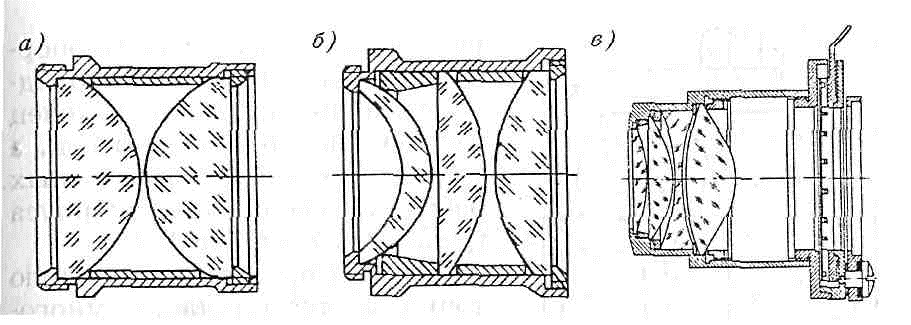
\includegraphics[width=1\textwidth]{5condensor.png}
	\label{pic:5condensor}
\end{figure}

\begin{figure}[h!]
	\caption{ Насыпная без промежуточных колец, конструкция фотообъектива }
	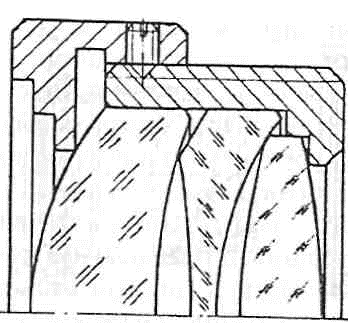
\includegraphics[width=0.4\textwidth]{5photoobj.png}
	\label{pic:5photoobj}
\end{figure}

Так как обеспечить высокую точность центрировки многокомпонентной линзовой системы из-за перечисленных погрешностей весьма сложно, а юстировка центрировки при насыпной конструкции затруднена или невозможна, то ее используют обычно в конструкциях осветительных систем (конденсоров, коллекторов), окуляров и относительно простых объективов. Данная конструкция не используется также в случаях, когда линзы системы существенно отличаются друг от друга по световому диаметру.

Насыпная конструкция (особенно без промежуточных колец) является наиболее технологичной, так как содержит минимально возможное количество деталей. Поэтому наблюдается устойчивая тенденция все более частого ее использования в конструкциях линзовых узлов приборов.

Насыпная в оправах конструкция отличается от предыдущей тем, что линзы и компоненты вначале закрепляются тем или иным способом (чаще всего завальцовкой или приклеиванием) в своих оправах, а затем устанавливаются последовательно в корпусную деталь (рис.~\ref{pic:5photoobj1},~\ref{pic:5photoobj2}).

\begin{figure}[h!]
	\caption{ Насыпная в оправах конструкция фотообъектива }
	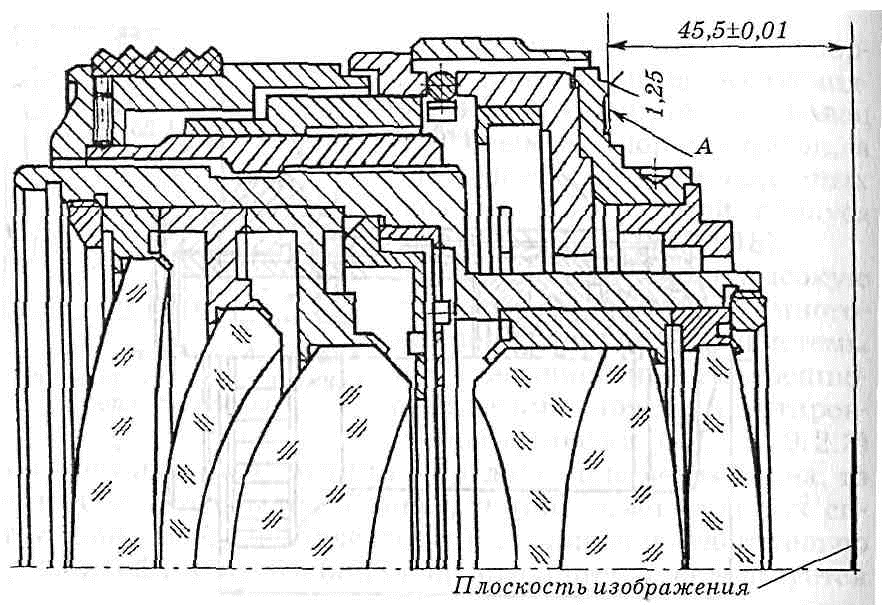
\includegraphics[width=1\textwidth]{5photoobj1.png}
	\label{pic:5photoobj1}
\end{figure}

\begin{figure}[h!]
	\caption{ Фотографический проекционный объектив }
	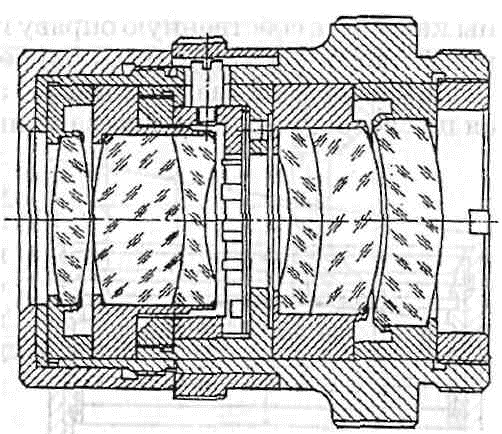
\includegraphics[width=1\textwidth]{5photoobj2.png}
	\label{pic:5photoobj2}
\end{figure}

Воздушные промежутки между компонентами обеспечиваются точным выполнением соответствующих конструктивных размеров оправ компонентов (при необходимости воздушный промежуток может юстироваться). Точность центрировки компонентов системы обуславливается погрешностями расположения центров кривизны их поверхностей и неперпендикулярностью плоских поверхностей относительно базовых осей оправ, зазорами посадок оправ в корпус, наклонами оправ из-за перекоса опорного торца корпуса и клиновидности оправ, несоосностью посадочных рабочих поверхностей корпуса (рис.~\ref{pic:5photoobj1}).

Насыпная в оправах конструкция применяется обычно при конструировании многокомпонентных фотобъективов (рис.~\ref{pic:5photoobj1}), микрообъективов, проекционных и фотограмметрических объективов (рис.~\ref{pic:5photoobj2}), зеркально-линзовых объективов.

На рис.~\ref{pic:5photoobj2} представлена конструкция многолинзового проекционного объектива, компоненты которого завальцованы каждый в собственную оправу и установлены в общий корпус. Силовое замыкание выполняется резьбовым кольцом.

В резьбовых конструкциях линзы и компоненты закрепляются каким-либо способом в своих оправах, которые соединяются по резьбе с корпусной деталью (рис.~\ref{pic:5photoobj3}).

\begin{figure}[h!]
	\caption{ Резьбовая конструкция оправы фотообъектива }
	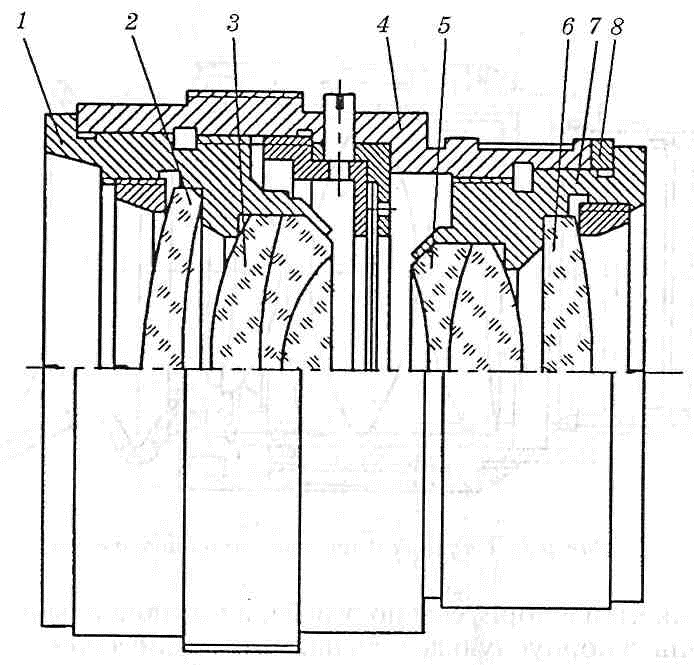
\includegraphics[width=0.8\textwidth]{5photoobj3.png}
	\label{pic:5photoobj3}
\end{figure}

Резьбовая конструкция является наименее технологичной из рассмотренных выше, так как более трудоемка при изготовлении и сборке, поэтому в настоящее время используется относительно других гораздо реже. В этой конструкции практически невозможно осуществлять юстировку центрировки компонентов системы.

В комбинированных конструкциях компоненты линзовых, систем сопрягаются с несущей (корпусной) деталью различными способами: непосредственно устанавливаются в корпус, насыпаются в оправах или их оправы соединяются с корпусом по резьбе (рис.~\ref{pic:5helios}).

На рис.~\ref{pic:5helios} изображена конструкция фотообъектива <<Гелиос-44Н>>, компоненты 1 и 2 которого закреплены в оправе, соединяемой с корпусом по резьбе, а компоненты 3 и 4 установлены в корпусную деталь насыпным способом. 

На рис.~\ref{pic:5Canon} изображена конструкция фотообъектива Canon, в которой присутствуют рассмотренные ранее различные конструкции крепления линз.

В специальных конструкциях линзы и компоненты устанавливаются и закрепляются в корпусной детали нетрадиционным способом. На рис.~\ref{pic:5obj} представлена конструкция проекционного объектива, линзы которого (две из них 1 и 3 выполнены из полистирола, а третья 2 -- из силикатного стекла) установлены в призматических канавках литой пластмассовой общей оправы, выполненной из двух цилиндрических половинок 4, 5. Крепление линз осуществляется обжимом их половинками оправы, вставленной в корпусную деталь. Благодаря упругости тонких буртиков призматических канавок производится беззазорное сопряжение линз с оправой. Точность расположения линз достигается точным литьем элементов оправы.

Более подробные сведения о конструкциях тех или иных видов и типов линзовых систем: объективов (например, фотографических, телескопических, проекционных, микроскопических, зеркально-линзовых), окуляров, осветительных систем изложены в справочниках и специальной литературе.
\begin{landscape}
	
	\begin{figure}[h!]
		\caption{ Фотообъектив <<Гелиос-44Н>> }
		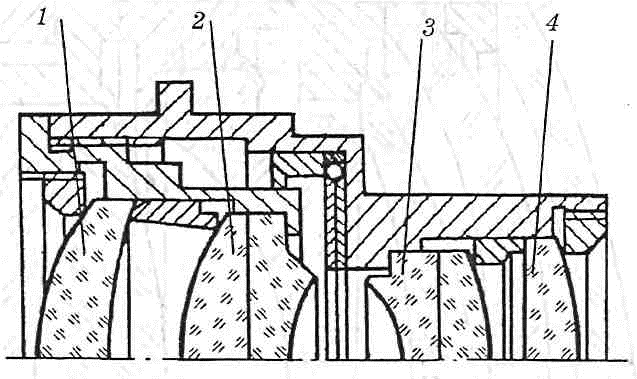
\includegraphics[width=0.45\textwidth]{5Helios.png}
		\label{pic:5helios}
	\end{figure}
	
	\begin{figure}[h!]
		\caption{ Фотообъектив Canon }
		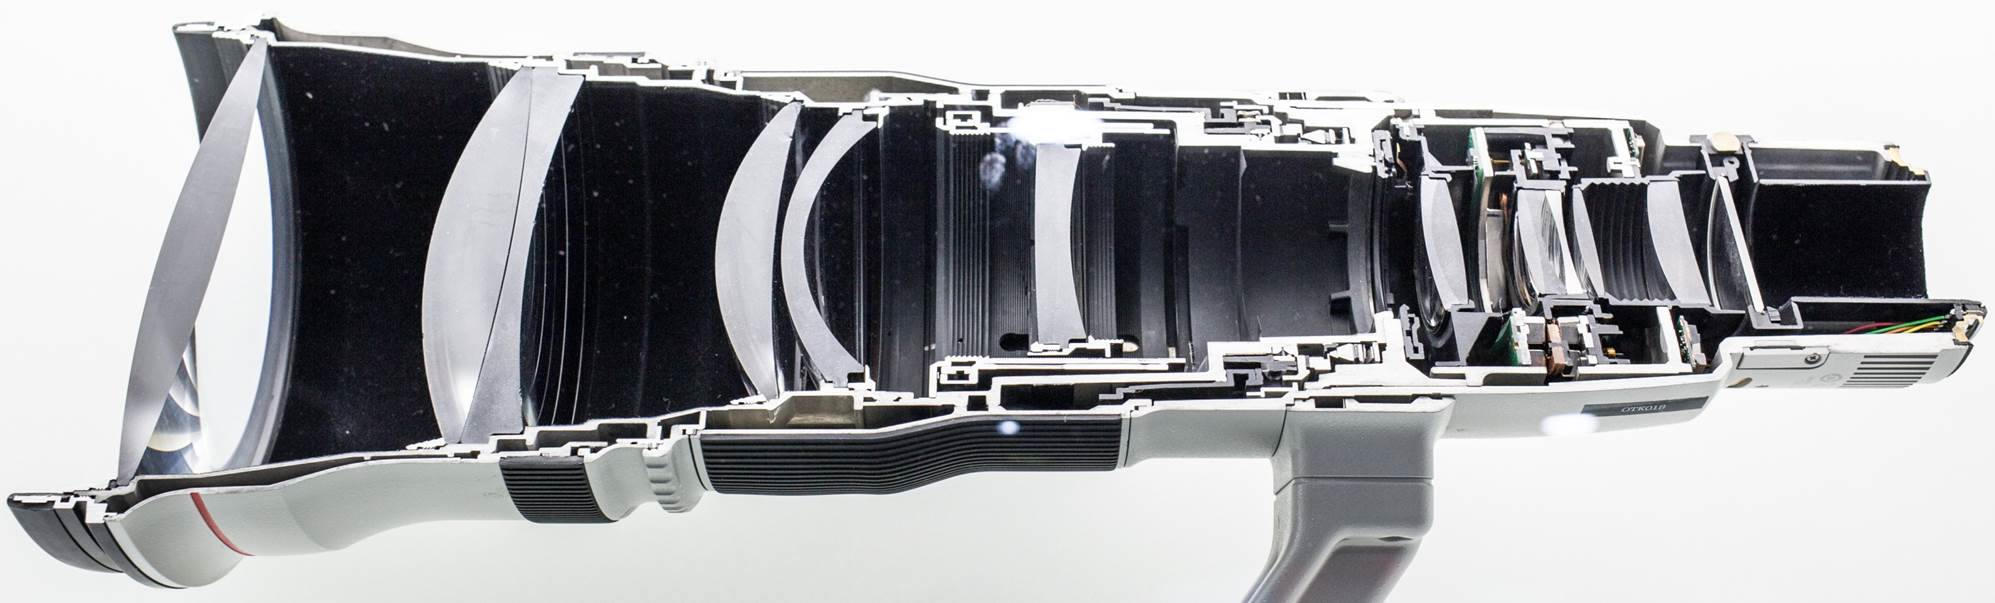
\includegraphics[width=0.9\textwidth]{5Canon.png}
		\label{pic:5Canon}
	\end{figure}
\end{landscape}

